\documentclass[tcc, capa]{texucpel}

%\usepackage[latin1]{inputenc} % acentuacao
\usepackage[utf8]{inputenc}
\usepackage[T1]{fontenc}
\usepackage{verbatim}
\usepackage{amsmath}
\usepackage{graphicx} % para inserir figuras

\usepackage{microtype} % detalhes de justificação e espaçamento
\usepackage{nowidow} % evita que a última linha de um parágrafo mude de pag.
\usepackage{paralist} % lista sem o espaçamento de uma linha entre itens
\usepackage{booktabs} % 'rules' em tabelas
\usepackage{multirow} % Mágicas com tabelas
\usepackage{amssymb} % checkmark
\usepackage{icomma} % corrigir decimais (exceto unidades SI)
\usepackage{fourier} % muda a fonte de matemática pra colidir menos com arial
\usepackage{nameref}
\usepackage{verbatim}
 \usepackage{float}
%\usepackage[tocindentauto]{tocstyle} % tentando fazer o apêndice funcionar

%\usepackage{color, soulutf8} % Revisão


%\usepackage{xcolor}
%\definecolor{text-gray}{gray}{0.08}

\usepackage{siunitx}

\sisetup{
	detect-family = true,
	detect-shape = true,
	detect-weight = true,
	detect-mode = true,
	output-decimal-marker = {,},
	binary-units = true
}%



\newcommand{\esp}{ESP8266}
\newcommand{\esppci}{ESP-01}
\newcommand{\exehda}{EXEHDA}
\newcommand{\middleware}{\emph{middleware}}
\newcommand{\pic}{PIC}
\newcommand{\picm}{PIC18F4550}
\newcommand{\picf}{PIC18F}
\newcommand{\hc}{HC-05}
\newcommand{\meter}{\mbox{ubiMeter}}

\newcommand{\gambi}{\fontfamily{phv}\fontshape{n}\selectfont}
\newcommand{\media}{\(\textrm{\gambi{} Média (\si{\volt})}\)}
\newcommand{\desvio}{\(\textrm{\gambi{} Desvio Padrão}\)}
\newcommand{\maximo}{\(\textrm{\gambi{} Máximo (\si{\volt})}\)}
\newcommand{\minimo}{\(\textrm{\gambi{} Mínimo (\si{\volt})}\)}
\newcommand{\erromed}{\(\textrm{\gambi{} Erro médio}\)}
\newcommand{\erromax}{\(\textrm{\gambi{} Erro máximo}\)}
%\(\textrm{\fontfamily{phv}\fontshape{n}\selectfont Média (\si{\volt})}\)

\unidade{Centro de Ciências Sociais e Tecnológicas}
\curso{Engenharia de Computação}
\nomecurso{Engenharia de Computação}
\titulocurso{Engenheiro de Computação.}

\title{Otimizando função de avaliação de docking molecular com uso de Redes Neurais}

\author{de Campos}{Gianluca}
%vspace{1.2cm}

\advisor [Prof. Me.]{Mertins}{Luciano Edson}
%\coadvisor [Prof.]{Sobrenome}{Nome}

\keyword{Otimização}
\keyword{Estrutura}
\keyword{Avaliação}

\begin{document}

%\color{text-gray}

\renewcommand{\advisorname}
{Orientador}           %descomente caso tenhas orientador
\renewcommand{\coadvisorname}{Coorientador}      %descomente caso tenhas coorientadora
\maketitle 

\sloppy

%\fichacatalografica

%\folhadeaprovacao

%Opcional
%\begin{dedicatoria}
%\end{dedicatoria}

%Opcional
%\begin{agradecimentos}
%\Agradecimentos:

%\vspace{\baselineskip}


%\end{agradecimentos}

%Opcional

%\begin{epigrafe}{Marilyn Manson}
 % "Sometimes I wonder if I'm a character being written, or if I'm writing myself."\\
%\end{epigrafe}

%\begin{epigrafe}{Neil Peart}
%"When the dust has cleared\\
%And victory denied\\
%A summit too lofty\\
%River a little too wide\\
%If we keep our pride -- \\
%Though paradise is lost\\
%We will pay the price,\\
%But we will not count the cost"\\
%\end{epigrafe}

%\begin{epigrafe}{Trey Anastasio, Tom Marshall}
%"But who can unlearn all the facts that I've learned\\
%As I sat in their chairs and my synapses burned\\
%And the torture of chalk dust collects on my tongue\\
%Thoughts follow my vision and dance in the sun\\
%All my vasoconstrictors they come slowly undone"\\
%\end{epigrafe}

%\begin{epigrafe}{Microchip}
%"bit TRISC<6> must be set (= 1)"\\
%\end{epigrafe}


% 1. Internet das coisas
% 2. Instrumentação virtual
% 3. Convergência
% 4. Proposta
% 5. Prototipação e cenários de teste

%Resumo em Portugues (no maximo 500 palavras)

\begin{comment}
O processo de desenvolvimento de fármacos é normalmente algo custoso financeiramente, que demanda muito tempo e recursos para serem realizados, muitas vezes é feito por uma pessoa de forma manual. 

Esta questão pode ser melhorada, caso todo o processo fosse automatizado computacionalmente, mais especificamente tendo, um software que examine a estrutura de uma célula ligante e também faça a comparação entre suas similaridades com outra célula, esta sendo chamda de receptora, afim de ter um mapeamento de moléculas  que definem  ambas estruturas das  duas células e também a avaliação do quanto estão bem ligadas, para isto é aplicada uma técnica, chamada de Docking Molecular.

Os softwares existentes, utilizam o docking para este processo de avaliação, porém, possuem um precisão de acertos imprecisos ao lidar com grandes volumes de dados para serem avaliados. 
Para que possa ser melhorada a precisão desses softwares, deve ser feito uma otimização na função de avaliação usado nestes sofwares e treina-la com deep learing, para que assim o processo de docking esteja trabalhando com melhores resultados. 
\end{comment}
\begin{abstract}
O processo de desenvolvimento de drogas medicinais é demorado,custoso e em grande parte manual.
Para melhorar e condicionar uma droga a um efeito desejado, utiliza-se uma técnica chamada Docking Molecular, que consiste em realizar atracamento de células e substâncias,onde o seu resultado demonstra o quão bem ligadas suas estruturas estão.Este processo é feito em grande parte por softwares, que exibem a melhor opção e combinações no design das células, ainda que estejam bem limitados em sua capacidade de predizer seus resultados.Uma possível solução seria utilizar Redes Neurais para otimizar este processo e diminuir o número de informações necessárias passadas para avaliação.
\end{abstract}

\begin{englishabstract}
  {Titulo do Trabalho em Inglês}
  {Algorithm, Optimization, Evaluation}  
  

The process of developing medicinal drugs is time-consuming, costly and largely manual.
In order to improve and condition a drug to a desired effect, a technique called Docking Molecular is used, which consists of docking of cells and substances, where its result demonstrates how well bound their structures are. \\
This process is largely done by softwares, which display the best choice and combinations in cell design, even though they are quite limited in their ability to predict their results.
A possible solution would be to use Neural Networks to optimize this process and decrease the number of information needed for evaluation.

\end{englishabstract}

%Lista de Figuras
\listoffigures

%Lista de Tabelas
\listoftables

\begin{listofabbrv}{RFCOMM}
		\item[UCPel] \textit{Universidade Cat\'olica de Pelotas}
        \item[CAPRI] \textit{Critical Assessment of PRedicted Interactions}

        
        
\end{listofabbrv}

%Sumario
\tableofcontents

\chapter{Introdução}
Ao ser desenvolvida uma nova droga é necessário estudar as propriedades químicas e analisar a estrutura das moléculas, o processo de desenvolvimento é bem custoso, pois leva tempo para poder realizar testes e avaliar resultados,que são feitos em vitro e examinados em laboratório sendo em grande parte manual e dependente de um ser humano.%\textbf{REF}%CITAR REFERENCIA DE COMO É FEITO DOCKING MANUALMENTE

Por consequência disso é comum que seja utilizado softwares que analizam estruturas celulares e aplicam a técnicas específicas da área de biomedicina, sendo uma delas o docking molecular, que ajuda a simular o comportamento entre duas estruturas ao se juntarem.
Com isto é possível poupar tempo e diminuir o custo de recursos no desenvolvimento de fármacos.

É de conhecimento geral que a tecnologia evoluiu muito nos ultimos anos, em especial na computação, tanto no software como no hardware,  em razão disso os programas que realizam docking hoje em dia tem cada vez maior capacidade para processamento, permitindo que seja obtido melhores resultados, desempenho e maior riquezas de detalhes ao explorar uma estrutura celular por exemplo, que pode ser vista de forma tridimensional.

Esses detalhes são importantes para aplicar o docking, pois trazem bastante informação ao realizar o estudo do comportamento entre duas estruturas celulares, que geralmente costumam ser um sequenciamento de DNA ou uma proteína.%\textbf{REF} % citar exemplo

Este comportamento é util para o desenvolvimento de fármacos, podendo ajudar a estudar inibidores de um vírus por exemplo,  onde ao aplicar a técnica de docking foi possível descobrir substâncias que pudessem inibir o vírus Influenza\cite{ishikawa2011binding}.

A técnica de docking consiste em analisar duas estruturas de células e junta-las com a melhor conformidade de encaixe possível, sendo a partir disto, possível de analisar as propriedades em comum e estuda-las.

Para poder aplicar o docking é necessário conhecer a molécula ligante, qual o receptor que seria qual estrutura ela irá se ligar (proteína ou dna). Ao conhecer as estruturas, é avaliado qual o melhor ponto em que serão encaixadas e a quantidade de energia que será liberada ao ocorrer esta ligação.

Este processo de avaliação foi calculado através diversos algoritmos ao longo dos anos como; algoritmo genético \cite{holland1975adaptation}, Simulate Annealing \cite{kirkpatrick1984optimization} ,  algoritmo genético de Lamarca \cite{morris1998automated},  MonteCarlo \cite{caflisch1992monte} entre outros que foram tiveram evoluções ao longo dos anos. 

Dependendo do algoritmo utilizado, a precisão do resultado pode variar, assim como seu desempenho e rapidez para gera-lo.
Com a evolução da área computacional, novos estudos são feitos para obter dados com melhor desempenho, em particular a Deep Learning tem se mostrado útil para vários estudos na área de biomedicina conforme avaliado por \cite{korotcov2017comparison,mamoshina2016applications}
, esta técnica basicamente consiste em treinar a máquina, para que ela possa classificar algo em grande escala afim de se obter da melhor forma possível  os resultados.


\section{Objetivo do trabalho}
Tendo em vista que o processo de desenvolvimento de fármacos é custoso, demorado e geralmente necessita de monitoramento, é necessário utilizar algum software que utilize a técnica de docking molecular para automatizar o processo.

O problema é que nem sempre os resultados gerados pela avaliação dos softwares são rápidos e precisos, essencialmente ao avaliar grandes volumes de dados.

Aproveitando a evolução de tecnologia que ocorreu tanto da área da biomedicina e computação, é possível otimizar o processo de docking utilizando técnicas de aprendizado de máquina, em especial, Redes Neurais Profundas (Deep Learning).

Esta mesma classificará da melhor forma a(s) função(oes) de avaliação, ao utilizar estruturas já conhecidadas em bases de dados e realizando a comparação.
Dividindo as etapas do docking em processos menores, ajudando a processar um volume de dados maior e também a ter melhores resultados.


\section{Organização do texto}
Neste trabalho foram dividivos da seguinte forma.
O Capítulo 2 abrange o referencial teórico sobre o qual será desenvolvido o trabalho de conclusão de curso, em específico, falará sobre a definição do que seria o docking, como é realizado o processo de docking, o contexto de onde está inserido, da mesma forma será feito ao falar sobre a Deep Learning.

No Capítulo 3, é apresentado como será realizado o estudo e otimização na avaliação do docking molecular ao aplicar Deep Learning, contendo uma descrição dos componentes necessários para fazê-la.

\chapter{Fundamentação Teórica}
Este capítulo faz uma breve revisão teórica sobre os assuntos necessários para a entender o processo de docking molecular  e deep learning.

\section{Docking Molecular}
No final da década de 1980, surgiram os primeiros softwares que realizavam o processo de docking molecular, possibilitando desta forma trazer uma visão mais detalhada das estruturas. Com isso foi possível manipular as moléculas e otimizar as células com mais facilidade e simular com maior precisão, permitindo mais rapidez ao realizar testes virtuais.

Para realizar o docking, é necessário realizar o mapeamento das proteínas que irão se ligar, isso serve para prever os melhores pontos para que as moléculas se liguem, e conhecendo assim o ponto com melhor conformidade e energia que será gasta para a união. Isto pode ser visto na figura 1, onde mostra duas protéinas realizando  docking e consequentemente gerando inúmeros pontos de conformidade.

      \begin{figure}[!htb]
	\centering
 \cite{xue2015protein}
    \caption{Exemplo de dockagem entre duas proteínas}
    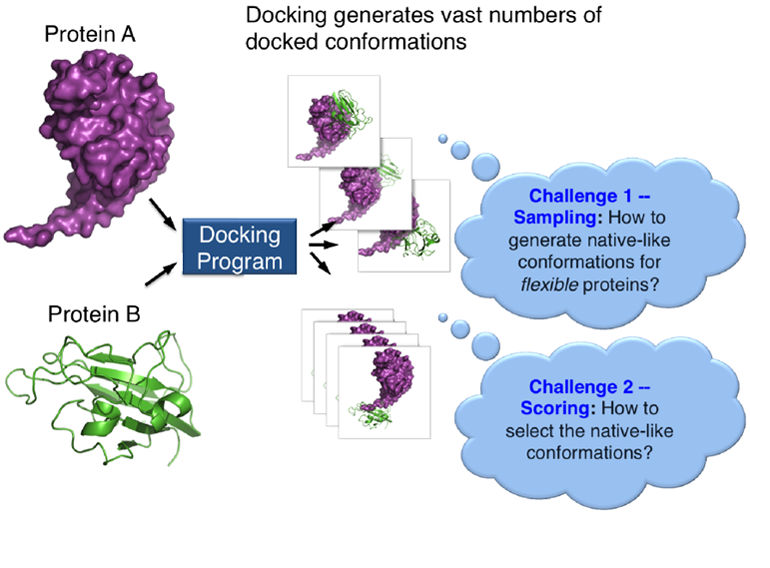
\includegraphics[width=10cm]{imagens/mostra_docking.png}
	\end{figure}
    
Tendo como objetivo analisar e prever a melhor conformidade entre duas estruturas celulares, conhecendo toda a região das moléculas das proteínas, ao aplicar o docking é possível descobrir a afinidade de ligação que estas duas moléculas possuem entre si, sendo assim estimando o melhor encaixe.
Ao ocorrer uma ligação, será liberado uma certa quantidade de energia, esta energia é importante para medir a conformidade da união entre duas moléculas (ligante e receptora).
Para realizar a medição, é utilizado funções de avaliação (score functions), focadas na minimização energética, que  segundo \cite{kitchen2004docking} e \cite{lybrand1995ligand}, chegaram a conclusão de que, quanto menor a energia gasta entre duas moléculas, melhor será sua a conformidade na união. 

Dependendo da estrutura que é analisada com o docking, torna-se possível criar uma substância capaz de inibir a molécula receptora, no caso de um inibidor de vírus por exemplo. \cite{ishikawa2011binding}

Com essa manipulação nas estruturas celulares, é possível destrinchar vários assuntos, pesquisas e artigos sobre os comportamentos de células e proteínas.
Esses exemplos são triviais para o estudo do comportamento das composições químicas das células para fazer medicamentos na aréa da biomedicina. 
Em geral é a técnica de docking molecular é utilizada para desenvolver estruturas de células diversas; vírus de doenças, medicamentos,dna e tudo que envolva fármacos. 

Muitos softwares já obtiveram resultados positivos ao utilizar docking, conforme mostrado na tabela 1 abaixo, onde é listado exemplos destes softwares.
\begin{table}[h]
\centering
\caption{Softwares bem sucedidos ao utilizar docking molecular \cite{sliwoski2014computational} }

\begin{tabular}{@{}|c|c|c|@{}}
\toprule

Software & Alvo                   & Estudo                                                   \\ \midrule
Seed     & Plasmepsin             & Uma das causas da malária                                \\ \midrule
FlexX    & Fator de Edema Anthrax & Inibidor do edema                                        \\ \midrule
Glide    & Citocromo P450         & Deixa substâncias em formas hidrosolúveis         \\ \midrule
Surflex  & Topoisomerase I        & Otimização de anti-cancerígeno                           \\ \midrule
Dock     & Imunofilina F506       & Inibidor de calcineurina \\ \bottomrule
\end{tabular}
\end{table}

Para \cite{rodrigues2012estrategias}, o objetivo principal que se tem ao aplicar docking é; aprimorar o processo de busca de novos candidatos a fármacos e acelerar o processo contínuo do seu planejamento. 
Todos os fatores como as propriedades químicas das moléculas auxiliam a compreender de qual maneira se comportará as células, quais os tipos de ligação que podem ser utilizados como; proteína-ligando, proteína-dna, proteína-proteína. Isso pode influenciar na abordagem de docking e afetar o desempenho nos softwares utilizados, ao serem aplicadas funções de pontuação.

Quanto a abordagem, existem duas formas diferentes de realizar o docking, que pode ser classificado como Docking Rígido e Docking Flexível.

No docking rígido os pontos de união de uma molécula ligante e receptora são mais limitados, isso se deve ao fato de existir uma menor liberdade em manipular as moléculas de uma célula, ou seja, a molécula ligante será rígida assim como o receptor. Consequentemente isso acaba resultando em maiores pontos a serem estimados para realizar a união de uma forma compatível. \\
Isso pode aumentar a precisão de acertos, já que existe vários pontos a serem avaliados e qual deles terá menor energia para realizar o acoplamento \cite{pagadala2017software}. 
Já no Docking Flexível, a molécula ligante pode ser manipulada com total liberdade ao tentar se acoplar no receptor,  este que continuará sendo rígido. O número de pontos a ser estimado será menor por ser ajustado a mólecula ligante ao receptor rígido.
Geralmente é utilizado esta abordagem após ser feito o docking rígido, orientado o melhor resultado estimado anteriormente para que desta forma tenha-se uma boa conformidade, isto é ilustrado na figura 2.


      \begin{figure}[!htb]
	\centering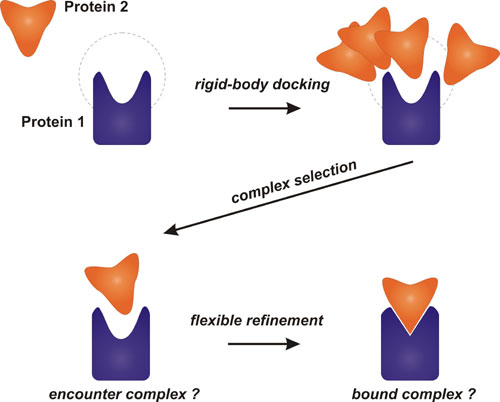
\includegraphics[width=10cm]{imagens/rigid_flexible.jpg}
	\caption{Docking Rígido com refinamento flexível}
	\end{figure}


\section{Função de pontuação}

O aprendizado de máquina se tornou algo bem comum ao ser aplicado em diversas áreas da computação, ao ser aplicado em software deve ser levantado os pontos que são relevantes para o processo de docking.

Nos softwares de docking são utilizados algoritmos para gerar funções de avaliação para estimar o gasto energético durante a união entre moléculas, como por exemplo algoritmo genético \cite{holland1975adaptation}, Simulate Annealing \cite{kirkpatrick1984optimization} ,  algoritmo genético de Lamarca \cite{morris1998automated},  MonteCarlo \cite{caflisch1992monte}.

Estes algoritmos estão constantemente sendo evoluídos e até substituídos para obterem mais eficácia ao estimar grandes volumes de dados com um desempenho melhor.

\section{Aprendizado de máquina }

Começando pelo pelo básico da IA, temos o aprendizado supervisionado e não supervisionado, dentre estes são utilizados funções de classificação e agregação que são muito limitadas para serem exploradas em um volumes de dados muito grande.
Para estudar o comportamento de uma célula é necessário fazer um mapeamento de sua estrutura para compreender suas peculiaridades e comportamentos. Tal processo é muito custuso e demorado dependendo do poder de processamento. 
Para fazer a máquina explorar toda a estrutura das móleculas, será requerido várias  bases de dados, com volumes grandiosos de informação. 

O foco será direcionado para o estudo de uma das técnicas de Inteligência Artificial na literatura, sendo uma delas redes neurais profundas, onde é possível utiliza-la para treinar os algoritmos para previsão e definição dos melhores resultados possíveis. 


\chapter{Metodologia}

Em primeiro momento o foco será estudar e fazer uma revisão bibliográfica a respeito do tema de Docking Molecular.

Esta revisão tem como objetivo se aprofundar nos temas que envolvem todo o processo de docking como onde é aplicado, qual o processo para ser executado, as ferramentas, requisitos necessários  e saber quais os resultados esperados computacionalmente.

A parte de aplicações refere-se ao uso de docking e para o que é útil,  em especial o que seria necessário para desenvolver algum fármaco.

O processo de realizar docking através de softwares ajuda a entender como ocorre o funcionamento desta técnica, com isso é possível saber ter uma estimativa de quais são os requisitos e resultados esperados que serão avaliados computacionalmente.
Após ser estudado o docking será realizado pesquisa a respeito da área de aprendizado de máquina, buscando especificamente o conhecimento da técnica de Redes Neurais Profundas que aborda temas como o a classificação das estruturas de proteínas bem como a predição dos melhores pontos estimados do docking.

Também deverá ser feito um levantamento das ferramentas de quais ferramentas (softwares) são utilizados e quais foram as otimizações das funções de avaliação que tiveram ao longo dos anos e quais os benchmarks.

Será necessário também testar e utilizar softwares,bases de dados e  frameworks que auxiliem no desenvolvimento e treino do aprendizado de máquina.

\begin{comment}
\section{Subseção}

\chapter{Resultados}

\section{Subseção}

\chapter{Conclusões}

\section{Trabalhos Futuros}
\end{comment}

\bibliography{relatorio}
\bibliographystyle{abnt}

%\appendix

\end{document}

